\documentclass[a4paper]{article}
\usepackage[utf8]{inputenc}
\usepackage[russian,english]{babel}
\usepackage[T2A]{fontenc}
\usepackage[left=10mm, top=20mm, right=18mm, bottom=15mm, footskip=10mm]{geometry}
\usepackage{indentfirst}
\usepackage{amsmath,amssymb}
\usepackage[italicdiff]{physics}
\usepackage{graphicx}
\graphicspath{{images/}}
\DeclareGraphicsExtensions{.pdf,.png,.jpg}
\usepackage{wrapfig}
\usepackage{float}
\usepackage{subcaption}
\usepackage{enumitem}
\usepackage{caption}
\usepackage{booktabs}
\usepackage{array}
\captionsetup[figure]{name=Рисунок}
\captionsetup[table]{name=Таблица}

\title{\underline{Отчет о выполненой лабораторной работе 4.3.2}}
\author{Воронин Денис, Б04-407}

\begin{document}

\maketitle

\begin{center}
\textbf{\Large Дифракция света на ультразвуковой волне
в жидкости (Горизонтальная щель)}
\end{center}

\textbf{Цель работы:}  изучение дифракции света на синусоидальной акустической решётке и наблюдение фазовой решётки методом тёмного поля.\par

\textbf{Оборудование:} оптическая скамья, осветитель, светофильтры, конденсор, щель, два длиннофокусных объектива, кювета с водой, кварцевый излучатель с микрометрическим винтом, генератор УЗ-частоты, частотомер, линза, отсчётное устройство, микроскоп.
\par

\textbf{Аннотация:} Должны будем измерить координаты дифракционных полос, образующихся при дифракции света на акустической решётке, а
также определить период этой решётки методом тёмного поля. По результатам измерений рассчитать скорость ультразвука в воде.

\section{Теоретическая справка}
При прохождении ультразвуковой волны через жидкость в ней возникают периодические неоднородности коэффициента преломления, создается фазовая решетка, которую мы считаем неподвижной ввиду малости скорости звука относительно скорости света. Показатель
	преломления n изменяется по закону:
	
	\begin{equation}\label{}
	n = n_0 (1 + m \cos \Omega x)
	\end{equation}
	
	Здесь $ \Omega = 2 \pi / \Lambda $ --- волновое число для ультразвуковой волны, $ m $ --- глубина модуляции $ n $ $ (m \ll 1 $).
	
	Положим фазу $ \phi $ колебаний световой волны на передней стенке кюветы равной нулю, тогда на задней поверхности она равна:
	
	\begin{equation}\label{}
	\phi  = k n L = \phi_0 (1 + m \cos \Omega x)
	\end{equation}
	
	Здесь $ L $ --- толщина жидкости в кювете, $ k = 2 \pi / \lambda $ --- волновое число для света.
	
	После прохождения через кювету световое поле есть совокупность плоских волн, распространяющихся под углами $ \theta $, соответствующими максимумам в дифракции Фраунгофера:
	
\begin{equation}\label{}	
	\Lambda \sin \theta_m = m \lambda
\end{equation}

Этот эффект проиллюстрирован на рисунке 1.

	Зная положение дифракционных максимумов, по формуле (1) легко определить длину ультразвуковой волны, учитывая малость $ \theta $: $ \sin \theta \approx \theta \approx l_m /F  $, где $ l_m $ --- расстояние от нулевого до последнего видимого максимума, $ F $ --- фокусное расстояние линзы. Тогда получим:
	
	\begin{equation}\label{}
	 \Lambda = m \lambda F/ l_m 
	\end{equation}
	Скорость ультразвуковых волн в жидкости, где $ \nu $ --- частота колебаний излучателя:
	
\begin{equation}\label{}
	v = \Lambda \nu 
\end{equation}

\begin{figure}[H]
	\center{
\includegraphics[scale=0.7]{p1.png}}
  \caption{Эффект дифракции на ультразвуковой волне}
	\label{fig:image1}
\end{figure}

\section{Экспериментальная установка}
На рисунке изображена схема экспериментальной установки. Источник света Л с помощью конденсора К проецируется на входную щель $S$. Входная щель ориентирована горизонтально и прикрыта красным светофильтром Ф. Коллиматорный объектив $\text{О}_1$ посылает параллельный пучок на кювету с водой $С$. Излучатель Q создаёт УЗ-волну. Параллельный пучок света, дифграгируя на стоячей звуковой волне, образует дифракционную картину в фокальной плоскости $F$ камерного объектива $\text{О}_{2}$. Картину можно наблюдать в микроскоп М.
\begin{figure}[H]
	\center{
\includegraphics[scale=0.7]{p2.png}}
  \caption{Схема экспериментальной установки}
	\label{fig:image1}
\end{figure}

\textbf{Темное поле}\par

\begin{wrapfigure}{l}{0.7\textwidth}
  \centering
  
\includegraphics[width=0.5\textwidth]{p3.png}
  \caption{Наблюдение акустической решётки методом тёмного поля
}
  \label{fig:example}
\end{wrapfigure}
Попробуем теперь получить видимое изображение фазовой
акустической решётки. Для этого, прежде всего, необходимо получить
в поле зрения микроскопа изображение задней плоскости (считая по
ходу световых лучей) кюветы. Это достигается с помощью вспомога
тельной положительной линзы O, которую располагают на оптической
скамье за фокальной плоскостью объектива $O_{2}$.\par

Перемещая микроскоп вдоль оптической скамьи, фокусируют его на плоскость $P$, где расположено чёткое изображение $a'b'$ какого-либо предмета $ab$, вплотную прижатого к стенке кюветы. Ясно, что чисто фазовая акустическая решётка является невидимой.

Для наблюдения пространственной структуры фазовой решётки можно использовать методы \textit{фазового контраста} или \textit{тёмного поля}. Фазовую структуру можно сделать видимой при изменении фазы колебаний в центральном дифракционном максимуме на $\pm\pi/2$. Такой метод наблюдения носит название \textit{метода фазового контраста}. В настоящей работе используется другой способ получения видимого изображения решётки --- \textit{метод тёмного поля}, основанный на устранении центрального дифракционного максимума с помощью специального экрана. Как нетрудно показать, в поле зрения микроскопа будут наблюдаться чередующиеся светлые и тёмные полосы, причём расстояние между тёмными полосами соответствует смещению в плоскости кюветы на $\Lambda/2$. Таким образом, должно наблюдаться характерное для метода тёмного поля удвоение числа деталей рассматриваемой структуры.

\newpage

\section{Ход работы}

\section{Определение скорости ультразвука по дифракционной картине}

\textbf{1.} Собрали схему согласно рисунку 2, включили осветитель и максимально открыли входную щель.

\begin{figure}[H]
	\center{
\includegraphics[scale=0.07]{p4.jpg}}
  \caption{Схема экспериментальной установки}
	\label{fig:image1}
\end{figure}

Открытие щели: -129 мкм.

\begin{figure}[htbp]
  \centering
  \begin{minipage}{0.3\textwidth}
    \centering
    
\includegraphics[width=\linewidth]{p5.jpg}
    \caption{Изображение 1} % общая подпись к figure, но внутри minipage caption не будет работать как надо без дополнительных пакетов. Лучше использовать просто текст.
  \end{minipage}\hfill
  \begin{minipage}{0.3\textwidth}
    \centering
    
\includegraphics[width=\linewidth]{p6.jpg}
  \end{minipage}\hfill
  \begin{minipage}{0.3\textwidth}
    \centering
    
\includegraphics[width=\linewidth]{p7.jpg}
  \end{minipage}
  \caption{Настройка щели}
\end{figure}

\textbf{2.} Получим дифракционную картину:

\begin{figure}[H]
	\center{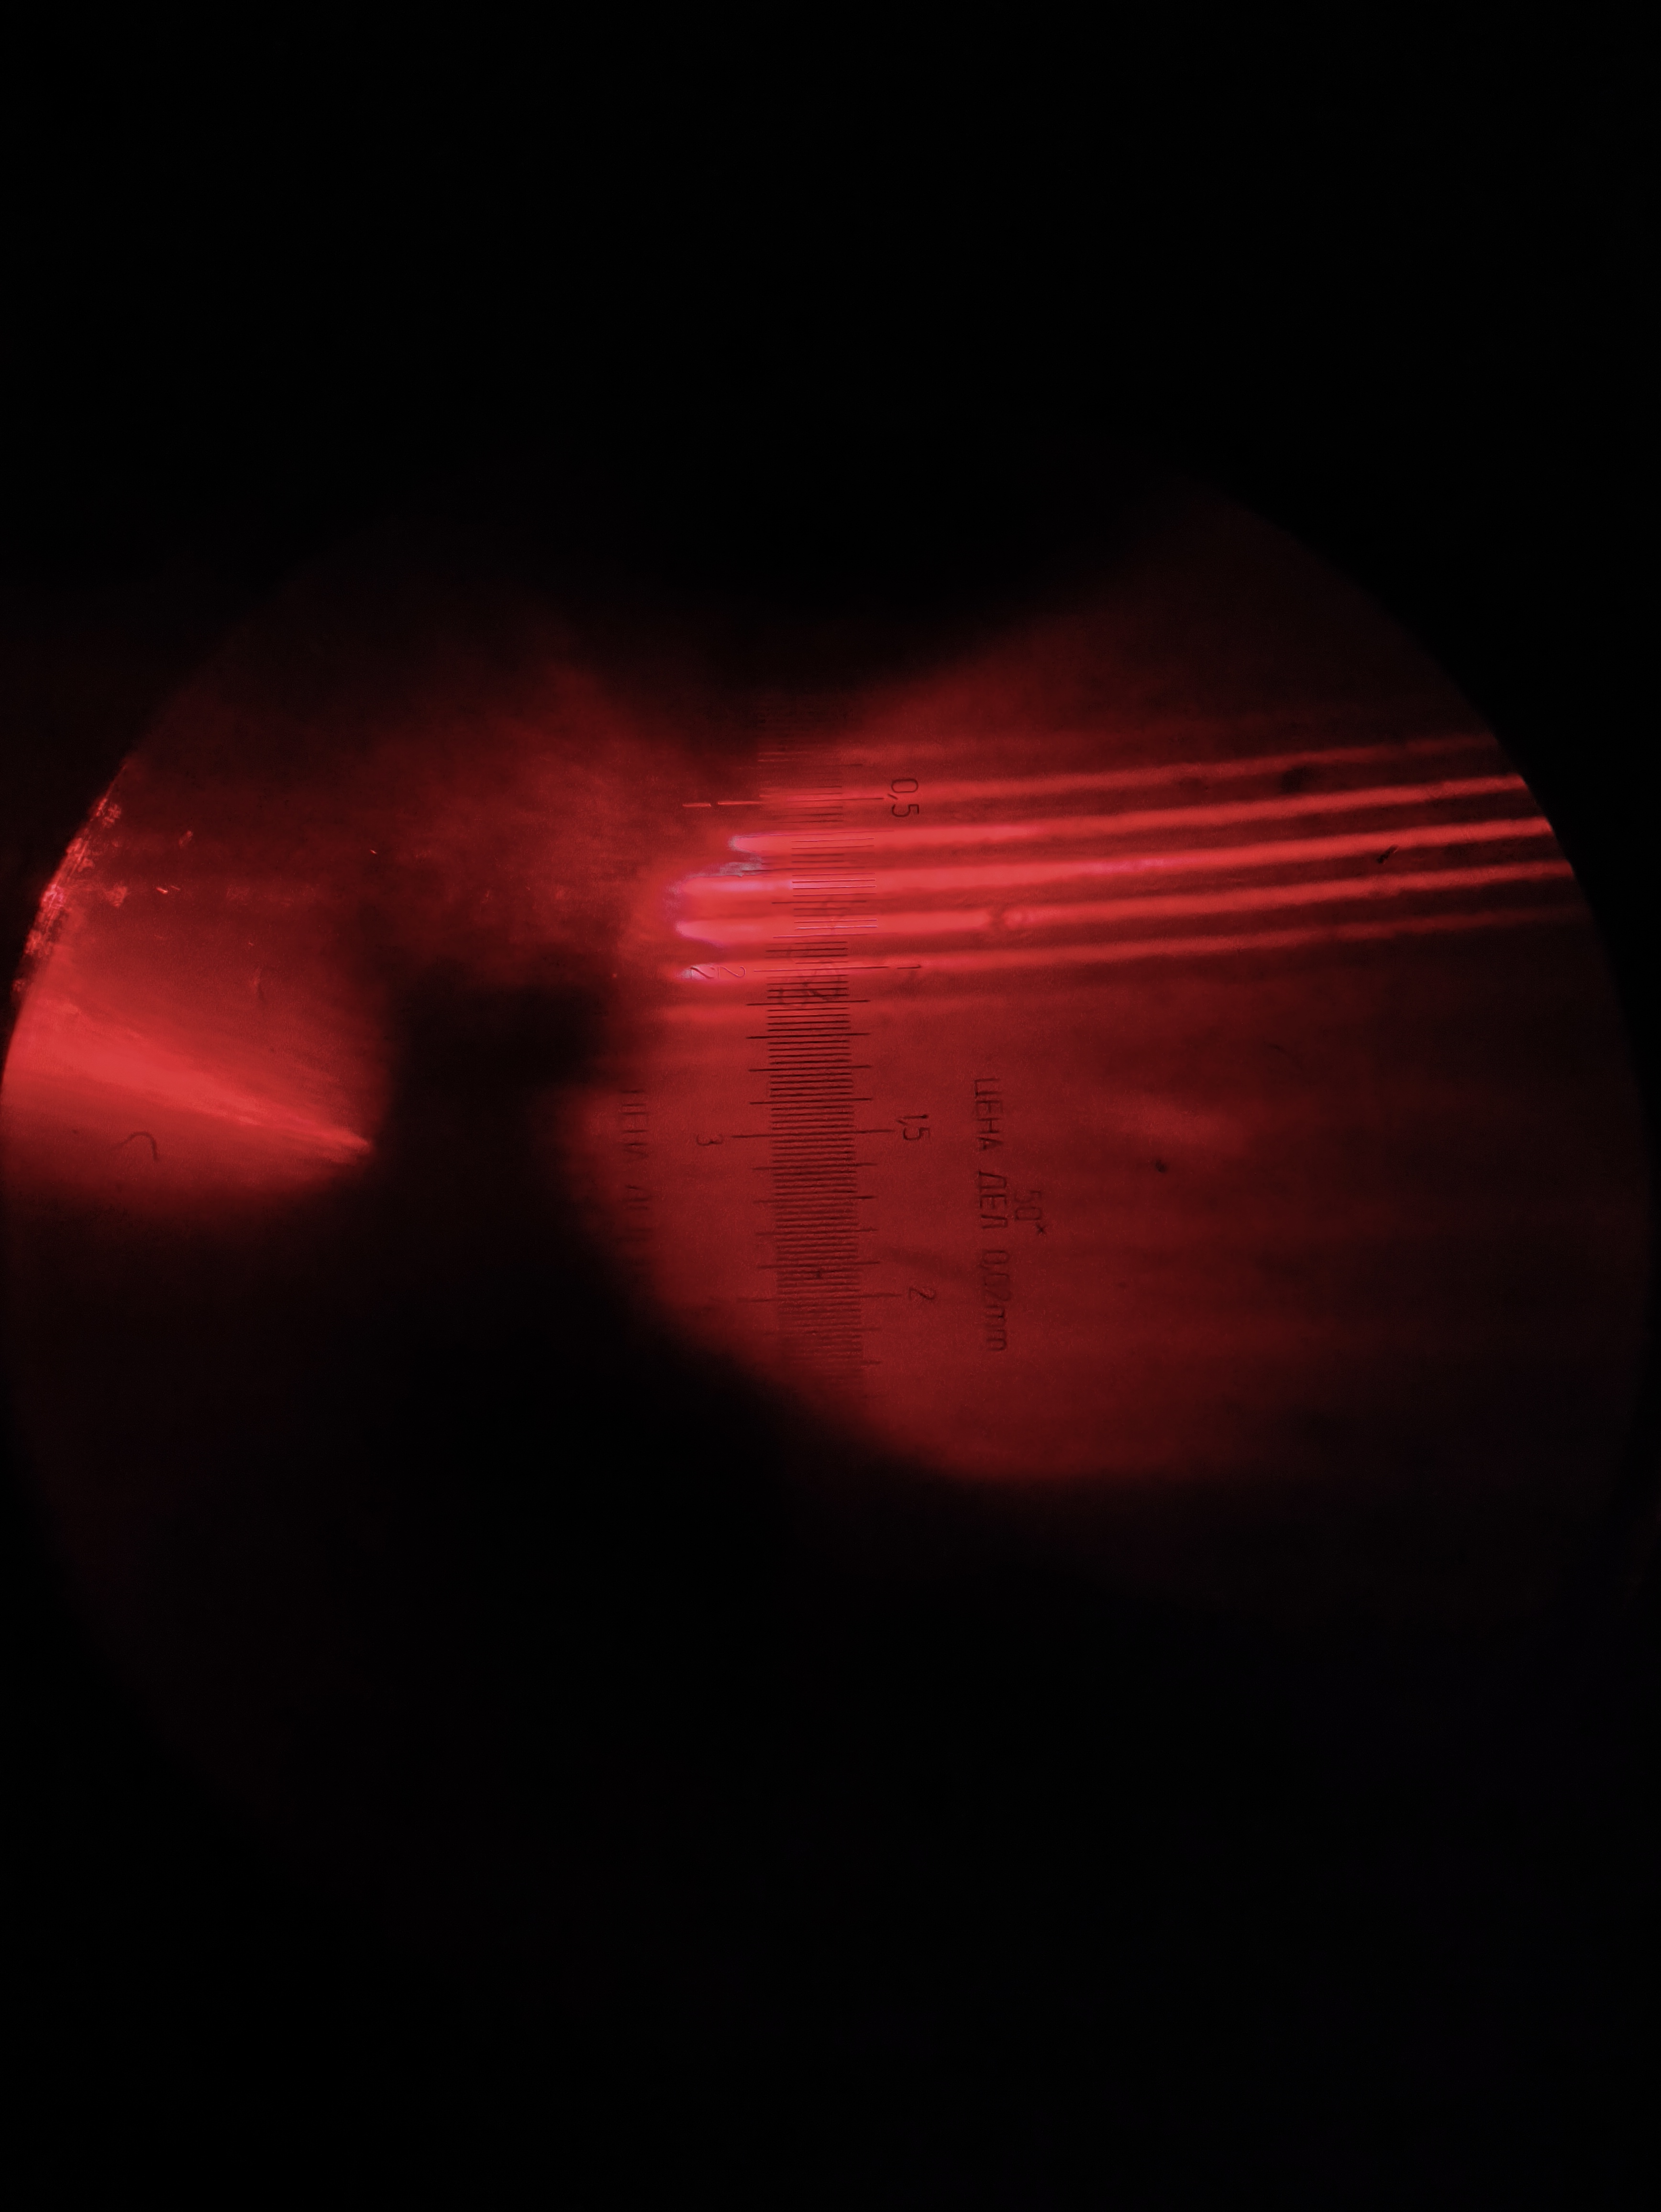
\includegraphics[scale=0.07]{p8.jpg}}
  \caption{Получение дифракционной картины}
	\label{fig:image1}
\end{figure}

Перемещая излучатель оценим по порядку величины длину УЗ-волны:\par

Расстояние между двумя полосами при частоте f = 6 МГц: $L = 0,12*2 = 0,24$\par

Вычислим скорость звука в воде: $\vartheta = \lambda * \nu = 0,00024*6*10^{6} = 1440$ м/c.

\textbf{3.} Определим положение дифракционных полос для нескольких частот:

Частота 1,0641 МГц

\begin{table}[htbp]
  \centering
  \begin{tabular}{|c|c|c|c|c|c|c|c|}
    \hline
    Номер полосы m & -3 & -2 & -1 & 0 & 1 & 2 & 3 \\
    \hline
    Координата мкм & -144 & -28 & 92 & 228 & 368 & 488 & 604 \\
    \hline
  \end{tabular}
%   \caption{Таблица 2×8 (8 столбцов, 2 строки)}
\end{table}

Частота 1,999 МГц

\begin{table}[htbp]
  \centering
  \begin{tabular}{|c|c|c|c|c|c|c|c|}
    \hline
    Номер полосы m & -2 & -1 & 0 & 1 & 2 & - & - \\
    \hline
    Координата мкм & 152 & 412 & 628 & 852 & 1100 & - & - \\
    \hline
  \end{tabular}
%   \caption{Таблица 2×8 (8 столбцов, 2 строки)}
\end{table}

Частота 4,4325 МГц

\begin{table}[htbp]
  \centering
  \begin{tabular}{|c|c|c|c|c|c|c|c|}
    \hline
    Номер полосы m & -1 & 0 & 1 & - & - & - & - \\
    \hline
    Координата мкм & 284 & 655 & 1028 & - & - & - & - \\
    \hline
  \end{tabular}
%   \caption{Таблица 2×8 (8 столбцов, 2 строки)}
\end{table}

\textbf{4.} Закроем проволочкой центральный максимум и запишем показания винта, перемещающего проволочку: $x_{\text{пр} = 60}$.

\textbf{5.} Построим график и из него получим коэффициенты наклона $l_{m}/m$.

Из нее по формулам $l_{m} = mf\frac{\lambda}{\Lambda} $ и $\vartheta = \Lambda \nu  $, где $\Lambda$ длина ультарзвуковой волны, а $\lambda$ длина используемой световой волны:

\begin{table}[htbp]
  \centering
  \caption{Экспериментальные данные}
  \begin{tabular}{|c|c|c|c|}
    \hline
    \(\nu\), МГц & \(l_m\), мкм & \(\Lambda\), мм & \(v\), м/с \\
    \hline
    1.080    & 126.86 & 1.41 $\pm 0.19$ & 1524 $\pm 31$ \\
    \hline
    1.936    & 233.60 & 0.77 $\pm 0.09$ & 1487 $\pm 25$\\
    \hline
    3.219    & 372.00 & 0.48 $\pm 0.7$ & 1549 $\pm 21$\\
    \hline
  \end{tabular}
\end{table}


\begin{figure}[H]
	\center{
\includegraphics[scale=0.7]{F1.png}}
  \caption{Зависимость расстояния между максимумами от номера}
	\label{fig:image1}
\end{figure}

Среднее значение $\vartheta = 1521$ м/с

Табличные значения $\Lambda$ для частоты 1 МГц: 1,5 мм \par
Табличные значения $\Lambda$ для частоты 2 МГц: 0,75 мм \par
Табличные значения $\Lambda$ для частоты 3 МГц: 0.5 мм \par

\section{Определение скорости ультразвука методом темного поля}

\textbf{1.} Поместим между щелью и микроскопом дополнительную линзу.
Поднимем излучатель и поместим в воду пластинку с калибровочной сеткой.\par

Расширим входную щель, чтобы увеличить поле зрения микроскопа. Передвигая микроскоп вдоль оптической оси настроимся на резкое изображение сетки в плоскости P. Цена малого деления окулярной шкалы составилала 0,1 мм.

\textbf{2.} Для наблюдения акустической решетки установим рабочую ширину щели 30 мкм. Уберем калибровочную метку из кюветы и опустим туда излучатель и постораемся увидеть звуковую решктку, меняя частоту в микроскоп.\par

\textbf{3.} Закроем нулевой максимум проволочкой.

\textbf{4.} Меняя частоту наблюдаем акустическую решетку.

\textbf{5.} Перемещая излучатель найдем наиболее четкую картину звуковой решетки и определим с помощью окулярной шкалы микроскопа координаты первой и последней видимых в поле зреения темный полос и количество светлых промежутков между ними для нескольких частот и посчитаем по формуле $\Lambda = 2* \frac{x_1-x_0}{m}$:

\begin{table}[htbp]
  \centering
  \caption{Экспериментальные данные}
  \begin{tabular}{|c|c|c|c|c|}
    \hline
    \(\nu\), МГц & \(x_0\), мм & \(x_1\), мм & \(m\) & \(\Lambda\), мм \\
    \hline
    1.28 & 5.0 $\pm 0.1$ & 6.4 $\pm 0.1$ & 2 & 1.41 $\pm 0.08$ \\
    \hline
    1.2235 & 4.8 $\pm 0.1$ & 6.0 $\pm 0.1$ & 2 & 1.17 $\pm 0.09$\\
    \hline
    1.5673 & 4.4 $\pm 0.1$ & 5.8 $\pm 0.1$ & 3 & 0.91 $\pm 0.09$ \\
    \hline
    2.0148 & 5.0 $\pm 0.1$ & 6.0 $\pm 0.1$ & 3 & 0.69 $\pm 0.09$ \\
    \hline
    2.1216 & 4.7 $\pm 0.1$ & 6.0 $\pm 0.1$ & 4 & 0.64 $\pm 0.10$ \\
    \hline
    4.4834 & 4.6 $\pm 0.1$ & 5.5 $\pm 0.1$ & 5 & 0.37 $\pm 0.10$\\
    \hline
  \end{tabular}
\end{table}

Построим график зависимости $\Lambda$ от $\frac{1}{\nu }$. По нему определим скорость ультразвука $\vartheta = 1628 \pm 76$ м/с.

\begin{figure}[H]
	\center{
\includegraphics[scale=0.7]{F2.png}}
  \caption{Зависимость $\Lambda$ от $\frac{1}{\nu }$}
	\label{fig:image1}
\end{figure}

\section{Вывод}
Были проведены измерения скорости ультразвука двумя разными способами:
\par
По дифракционной картине. Получены значения $v = 1524$ м/с, $v = 1487$ м/с, $v = 1549$ м/с и среднее $v = 1521$ м/с. \par
Измерения методом темного поля. Получено значения $v = 1628 \pm 76$ м/с.\par
Видим, что значение, полученное методом темного поля, сходится в пределах погрешности со средним значением, но не сходится с некоторыми отдельными значениями. Это может объясняться тем, что при измерении по дифракционной картине относительно велика погрешность измерений, так как эти измерения основываются на измерениях расстояния между дифракционными максимумаи, расстояние между которыми может быть неверно измерено.

\end{document}